% !TeX spellcheck = fr_FR
\chapter{Chapitre 3 : Implémentation Des Solutions}

Dans ce chapitre, je vais décrire le fonctionnement et l'implémentation des deux solutions dont j'ai parlé dans le chapitre deux.

\section{Description Solution UART}

Cette première solution va générer les mots de passe directement dans l’\gls{fpga}, ainsi, on aura besoin du communication \gls{uart} afin de paramétrer l’attaque depuis notre ordinateur. 
On va notamment pouvoir communiquer le hash et le salt que l’on souhaite casser, ainsi que l’état initial du générateur de mot de passe et le nombre d’essais avant d’arrêter l'attaque.

Cette communication nécessite un encodage permettant de délimiter les paquets, ainsi qu'un moyen de vérification d'erreurs afin de savoir si le paquet n'a pas subi des pertes en chemin.

\subsection{Encodage Cobs}

Une manière assez simple d’encoder un paquet et de le délimiter à l’aide de caractères spéciaux. 
C’est une méthode qui marche assez bien lorsque les données que l’on envoie sont limitées comme du texte par exemple. 
Toutefois, dans notre cas, nous souhaitons envoyer des données brutes qui peuvent contenir tout type de valeurs.

Il me fallait donc une méthode un peu plus poussée, c’est pour cela que je suis parti sur le \gls{cobs} qui est une méthode d’encodage assez légère et simple d’implémentation.

L’idée du \gls{cobs} est d’utiliser la valeur zéro comme indicatif de fin de paquet. 
Puis de remplacer tous les zéros présents dans le paquet d’origine par une valeur qui indique à combien d’octets, se trouve le prochain zéro. 
Un octet est ensuite ajouté au début du paquet pour indiquer la position du premier zéro dans les données originales. 
Ainsi, le paquet encodé ne contiendra qu’un seul zéro, situé à la fin, qui servira de marqueur pour indiquer la fin du paquet au destinataire. 
Au final, cette méthode est plutôt simple à mettre en place et rajoute seulement deux octets par rapport au paquet d’origine.

\begin{figure}[tbph!]
	\centering
	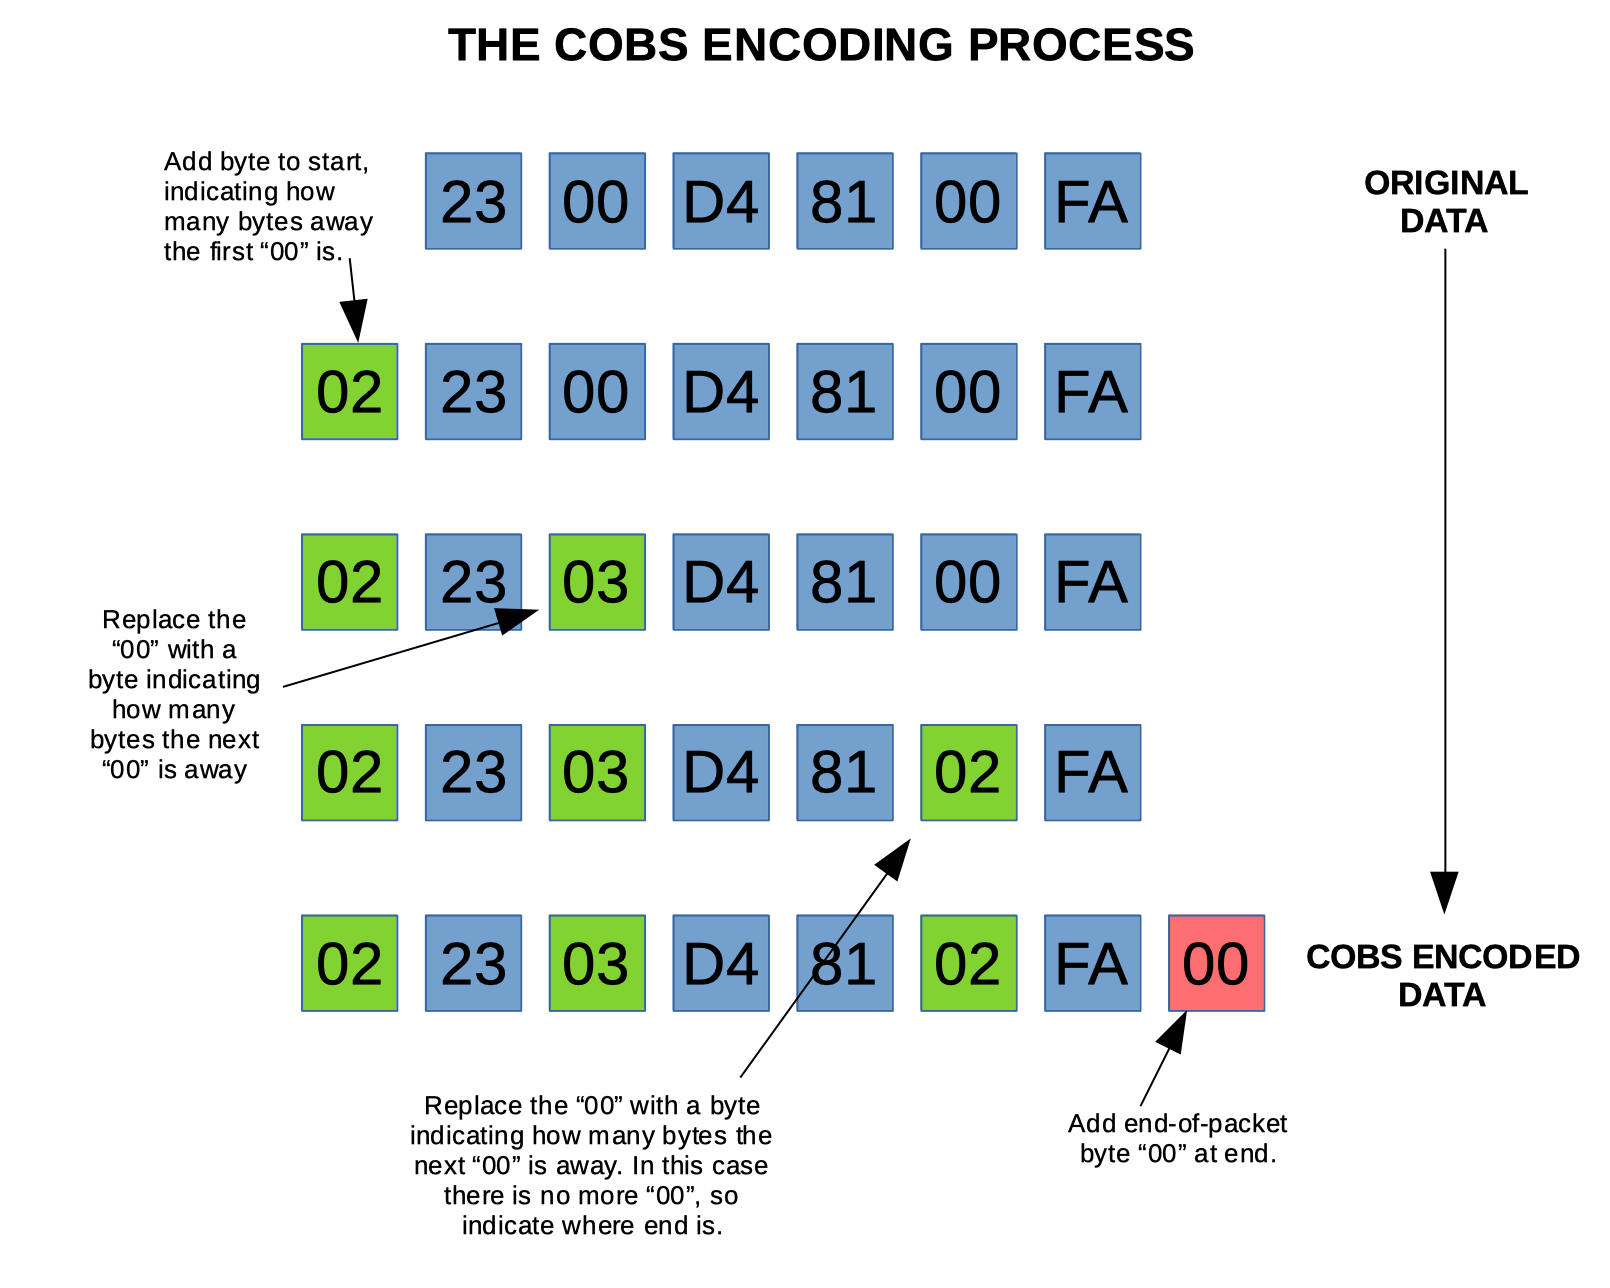
\includegraphics[width=0.7\linewidth]{cobs_encoding}
	\caption[Schéma Encodage COBS]{Schéma Encodage COBS. Source : blog.mbedded.ninja ref. URL02}
	\label{fig:cobs_encoding}
\end{figure}

\subsection{CRC}

Pour ce qui est de la vérification d'erreurs, l'algorithme utilisé de manière général est le \gls{crc}.
Après quelques recherches, je suis tombé sur un site internet\footcite{noauthor_generator_nodate} qui permet de générer du code dont du \gls{vhdl} en fonction du type de \gls{crc} souhaité.
Je suis parti sur le \gls{crc} le plus simple qui est le 8 bit, mais le code \gls{vhdl} nous est fourni sous forme de module, il est donc assez facile de remplacer le \gls{crc} par un autre plus rigide.

\newpage

\subsection{Format et Type de Paquet}

Au final, tous les paquets doivent être structurer dans le même format en prenant compte de l'encodage et du \gls{crc}. 
J'ai aussi pris l'initiative pour être sûr d'ajouter un champ supplémentaire dans le paquet qui est la taille du paquet d'origine, car le paquet provenant de l'ordinateur devrait toujours être de la même taille. 

\begin{figure}[tbph!]
	\centering
	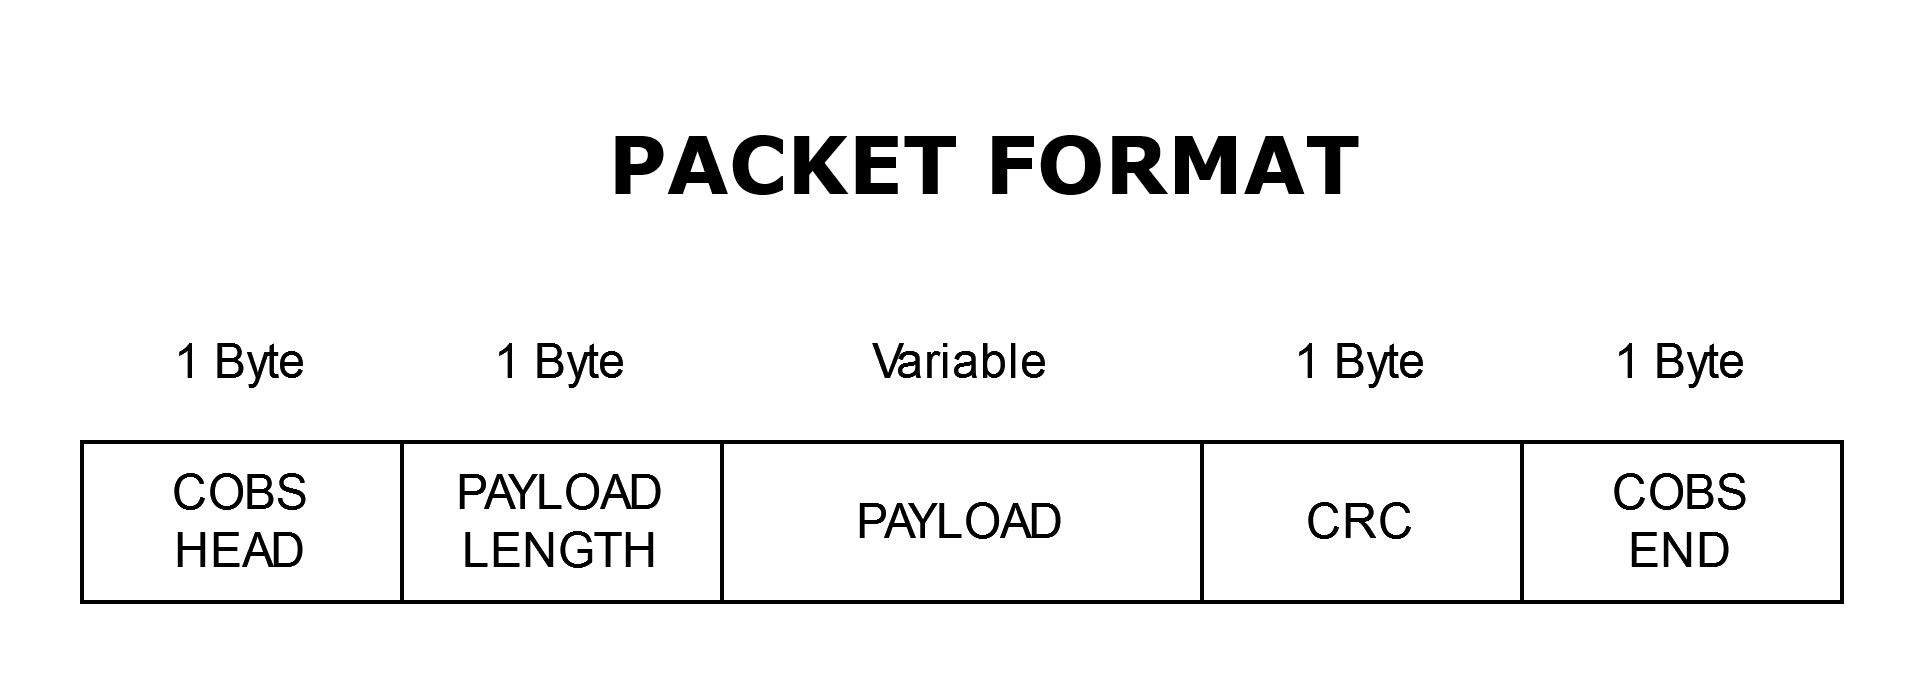
\includegraphics[width=0.6\linewidth]{uart_packet_format}
	\caption[Format de paquet - UART]{Format de paquet - UART. Source : réalisé par Kandiah Abivarman}
	\label{fig:uart_packet_format}
\end{figure}


\subsubsection{Paquet pour le FPGA}

Lorsque l'on souhaite faire une attaque, on doit envoyer un paquet pour configurer chaque quadcore.
De ce fait, on a qu'un seul type de paquet à envoyer et il faut en envoyer en fonction du nombre de quadcore présent dans le \gls{fpga}.

\begin{figure}[tbph!]
	\centering
	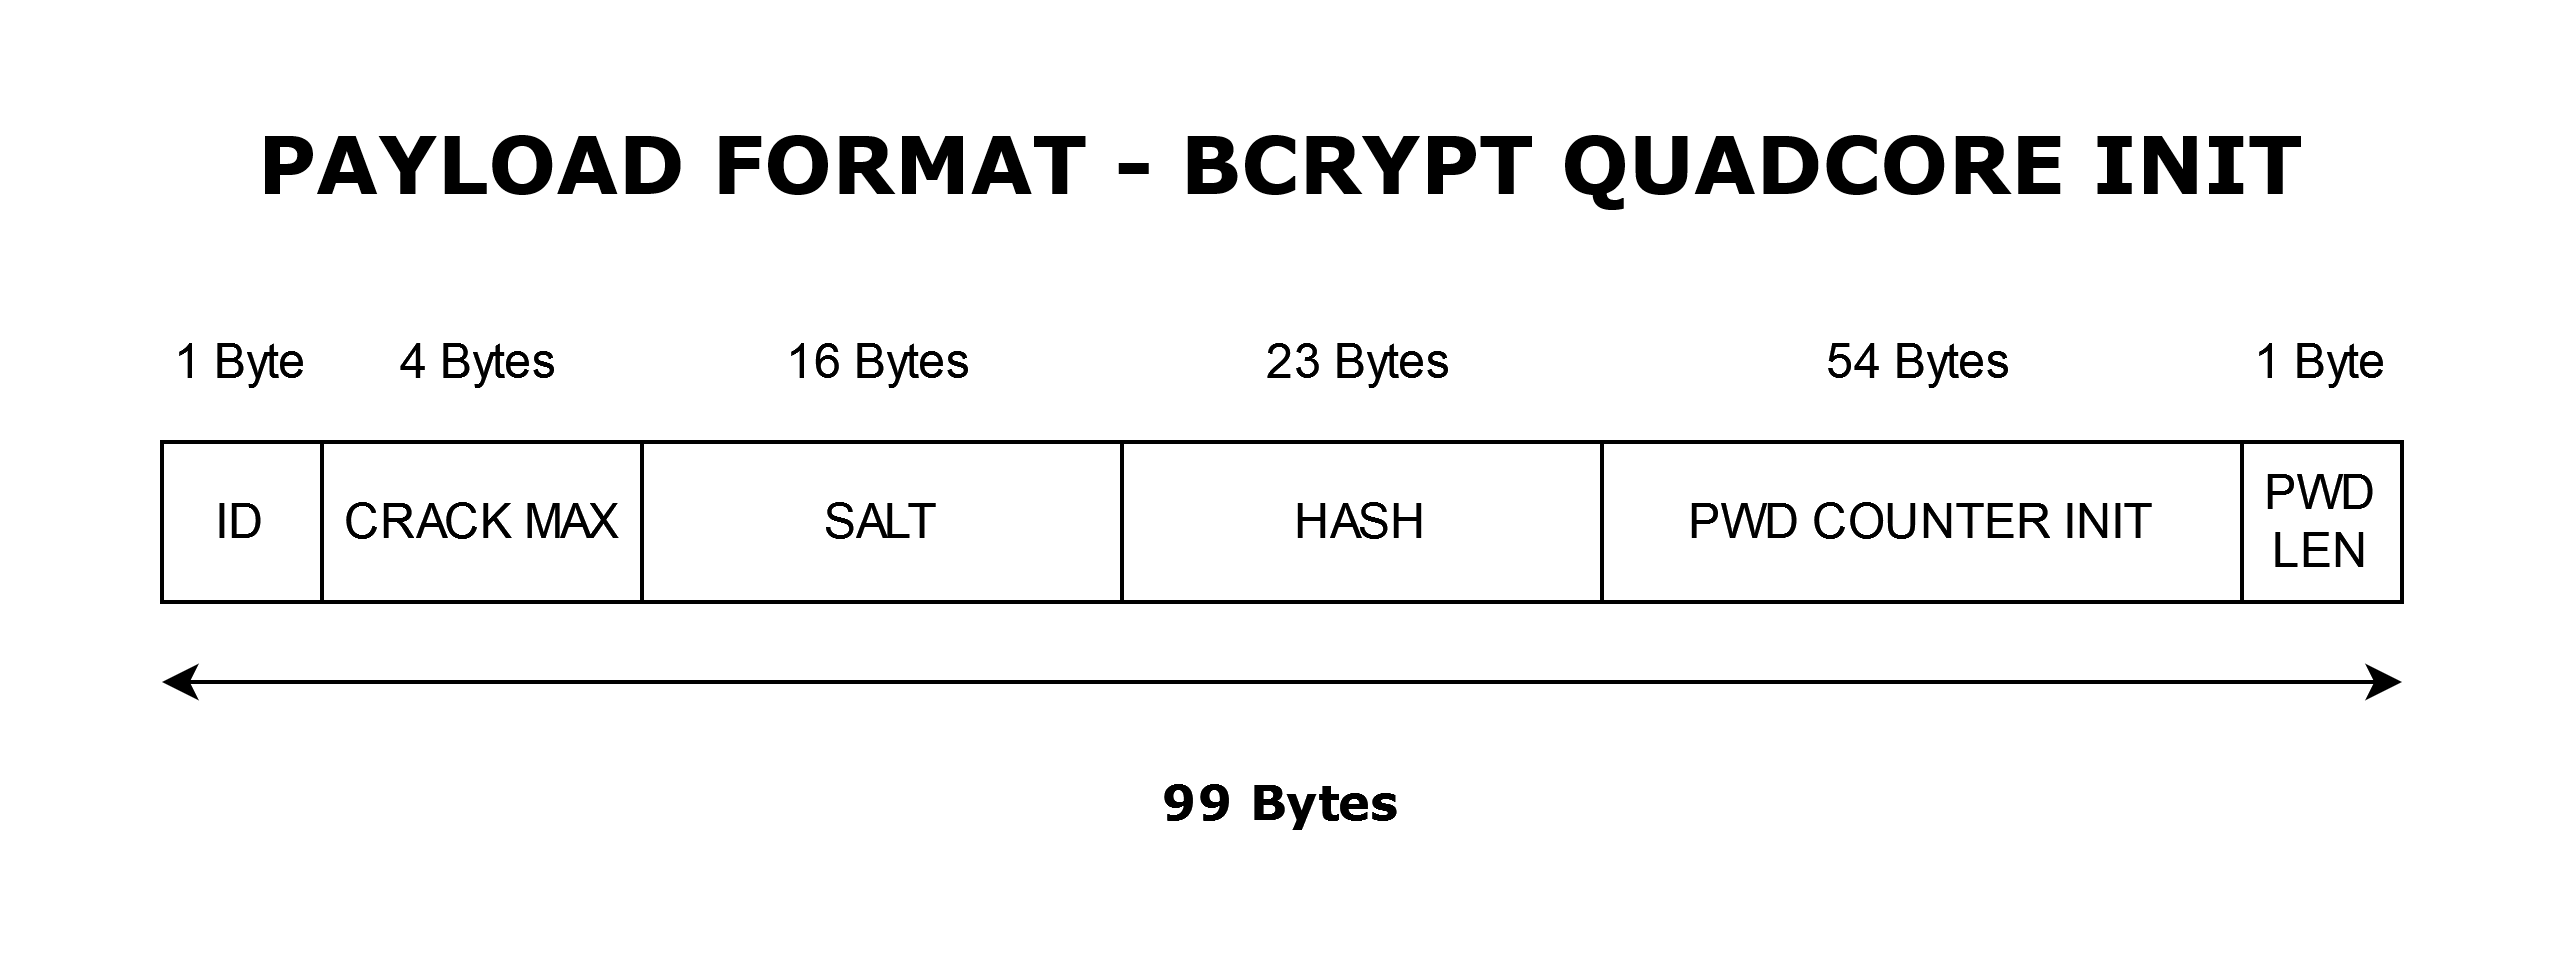
\includegraphics[width=0.7\linewidth]{uart_mosi_payload_format}
	\caption[Format de paquet - MOSI]{Format de paquet - MOSI. Source : réalisé par Kandiah Abivarman}
	\label{fig:uart_mosi_payload_format}
\end{figure}

\newpage

\subsubsection{Paquet pour l'ordinateur}

Lorsque le \gls{fpga} recevra un paquet, il devrait envoyer un paquet de réponse afin d'avertir l'ordinateur de la bonne réception du paquet.

\begin{figure}[tbph!]
	\centering
	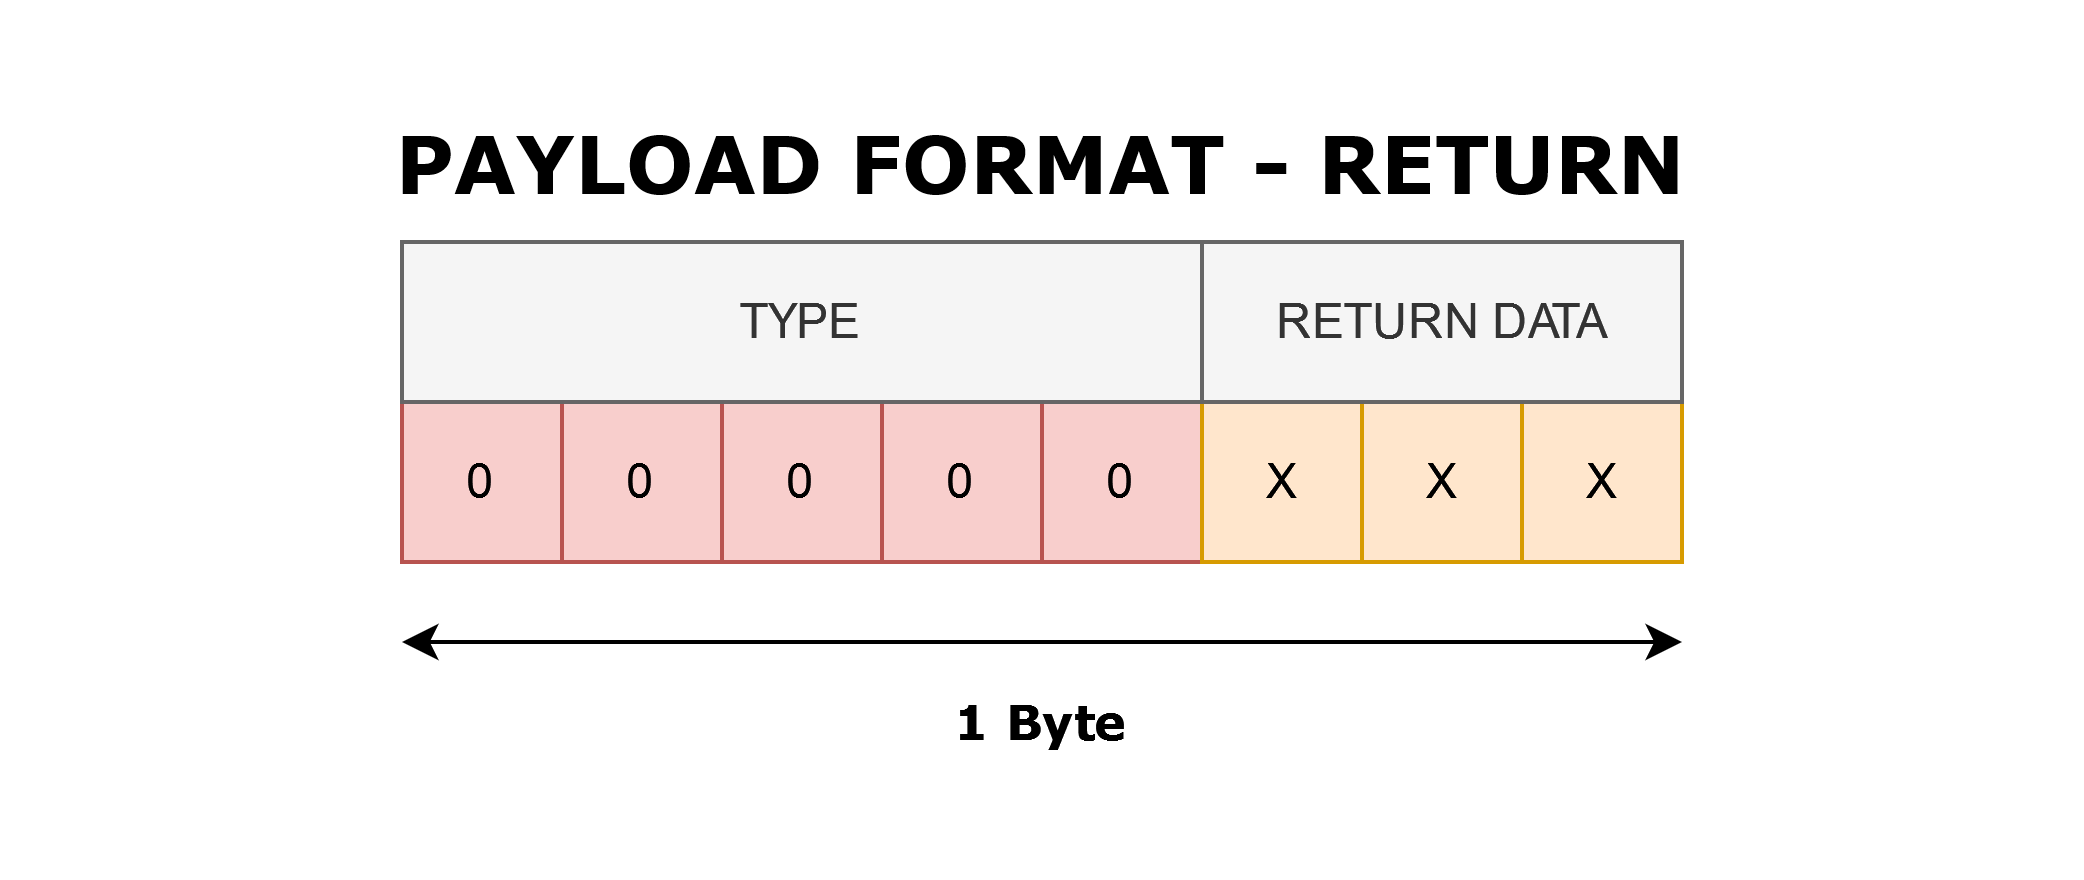
\includegraphics[width=0.7\linewidth]{uart_return_payload_format}
	\caption[Format de paquet - Retour]{Format de paquet - Retour. Source : réalisé par Kandiah Abivarman}
	\label{fig:uart_return_payload_format}
\end{figure}

Lorsque le paquet est une réponse, le champ type vaudra zéro est les trois bits de point faibles vont nous indiquer l'erreur si il y en a une.\\

\begin{table}[tbph!]
	\centering
	\begin{tabular}{|c|c|}
	\hline
	\textbf{Return Code} & \textbf{Return}                   \\ \hline
	000                  & OK                                \\ \hline
	001                  & Packet size greater than expected \\ \hline
	010                  & Packet size smaller than expected \\ \hline
	011                  & Quadcore ID not valid             \\ \hline
	100                  & CRC Error                         \\ \hline
	\end{tabular}
\end{table}

Quand le paquet n'est pas une réponse alors les trois bits vaudront zéros et pourront être ignoré. 

\newpage

En dehors d'une réponse, le \gls{fpga} envoyera aussi un paquet toutes les secondes pour donner l'état d'avancement de l'attaque.
Puis, bien évidemment un paquet sera aussi envoyer lorsque le mot de passe cherché sera trouvé.

\begin{figure}[tbph!]
	\centering
	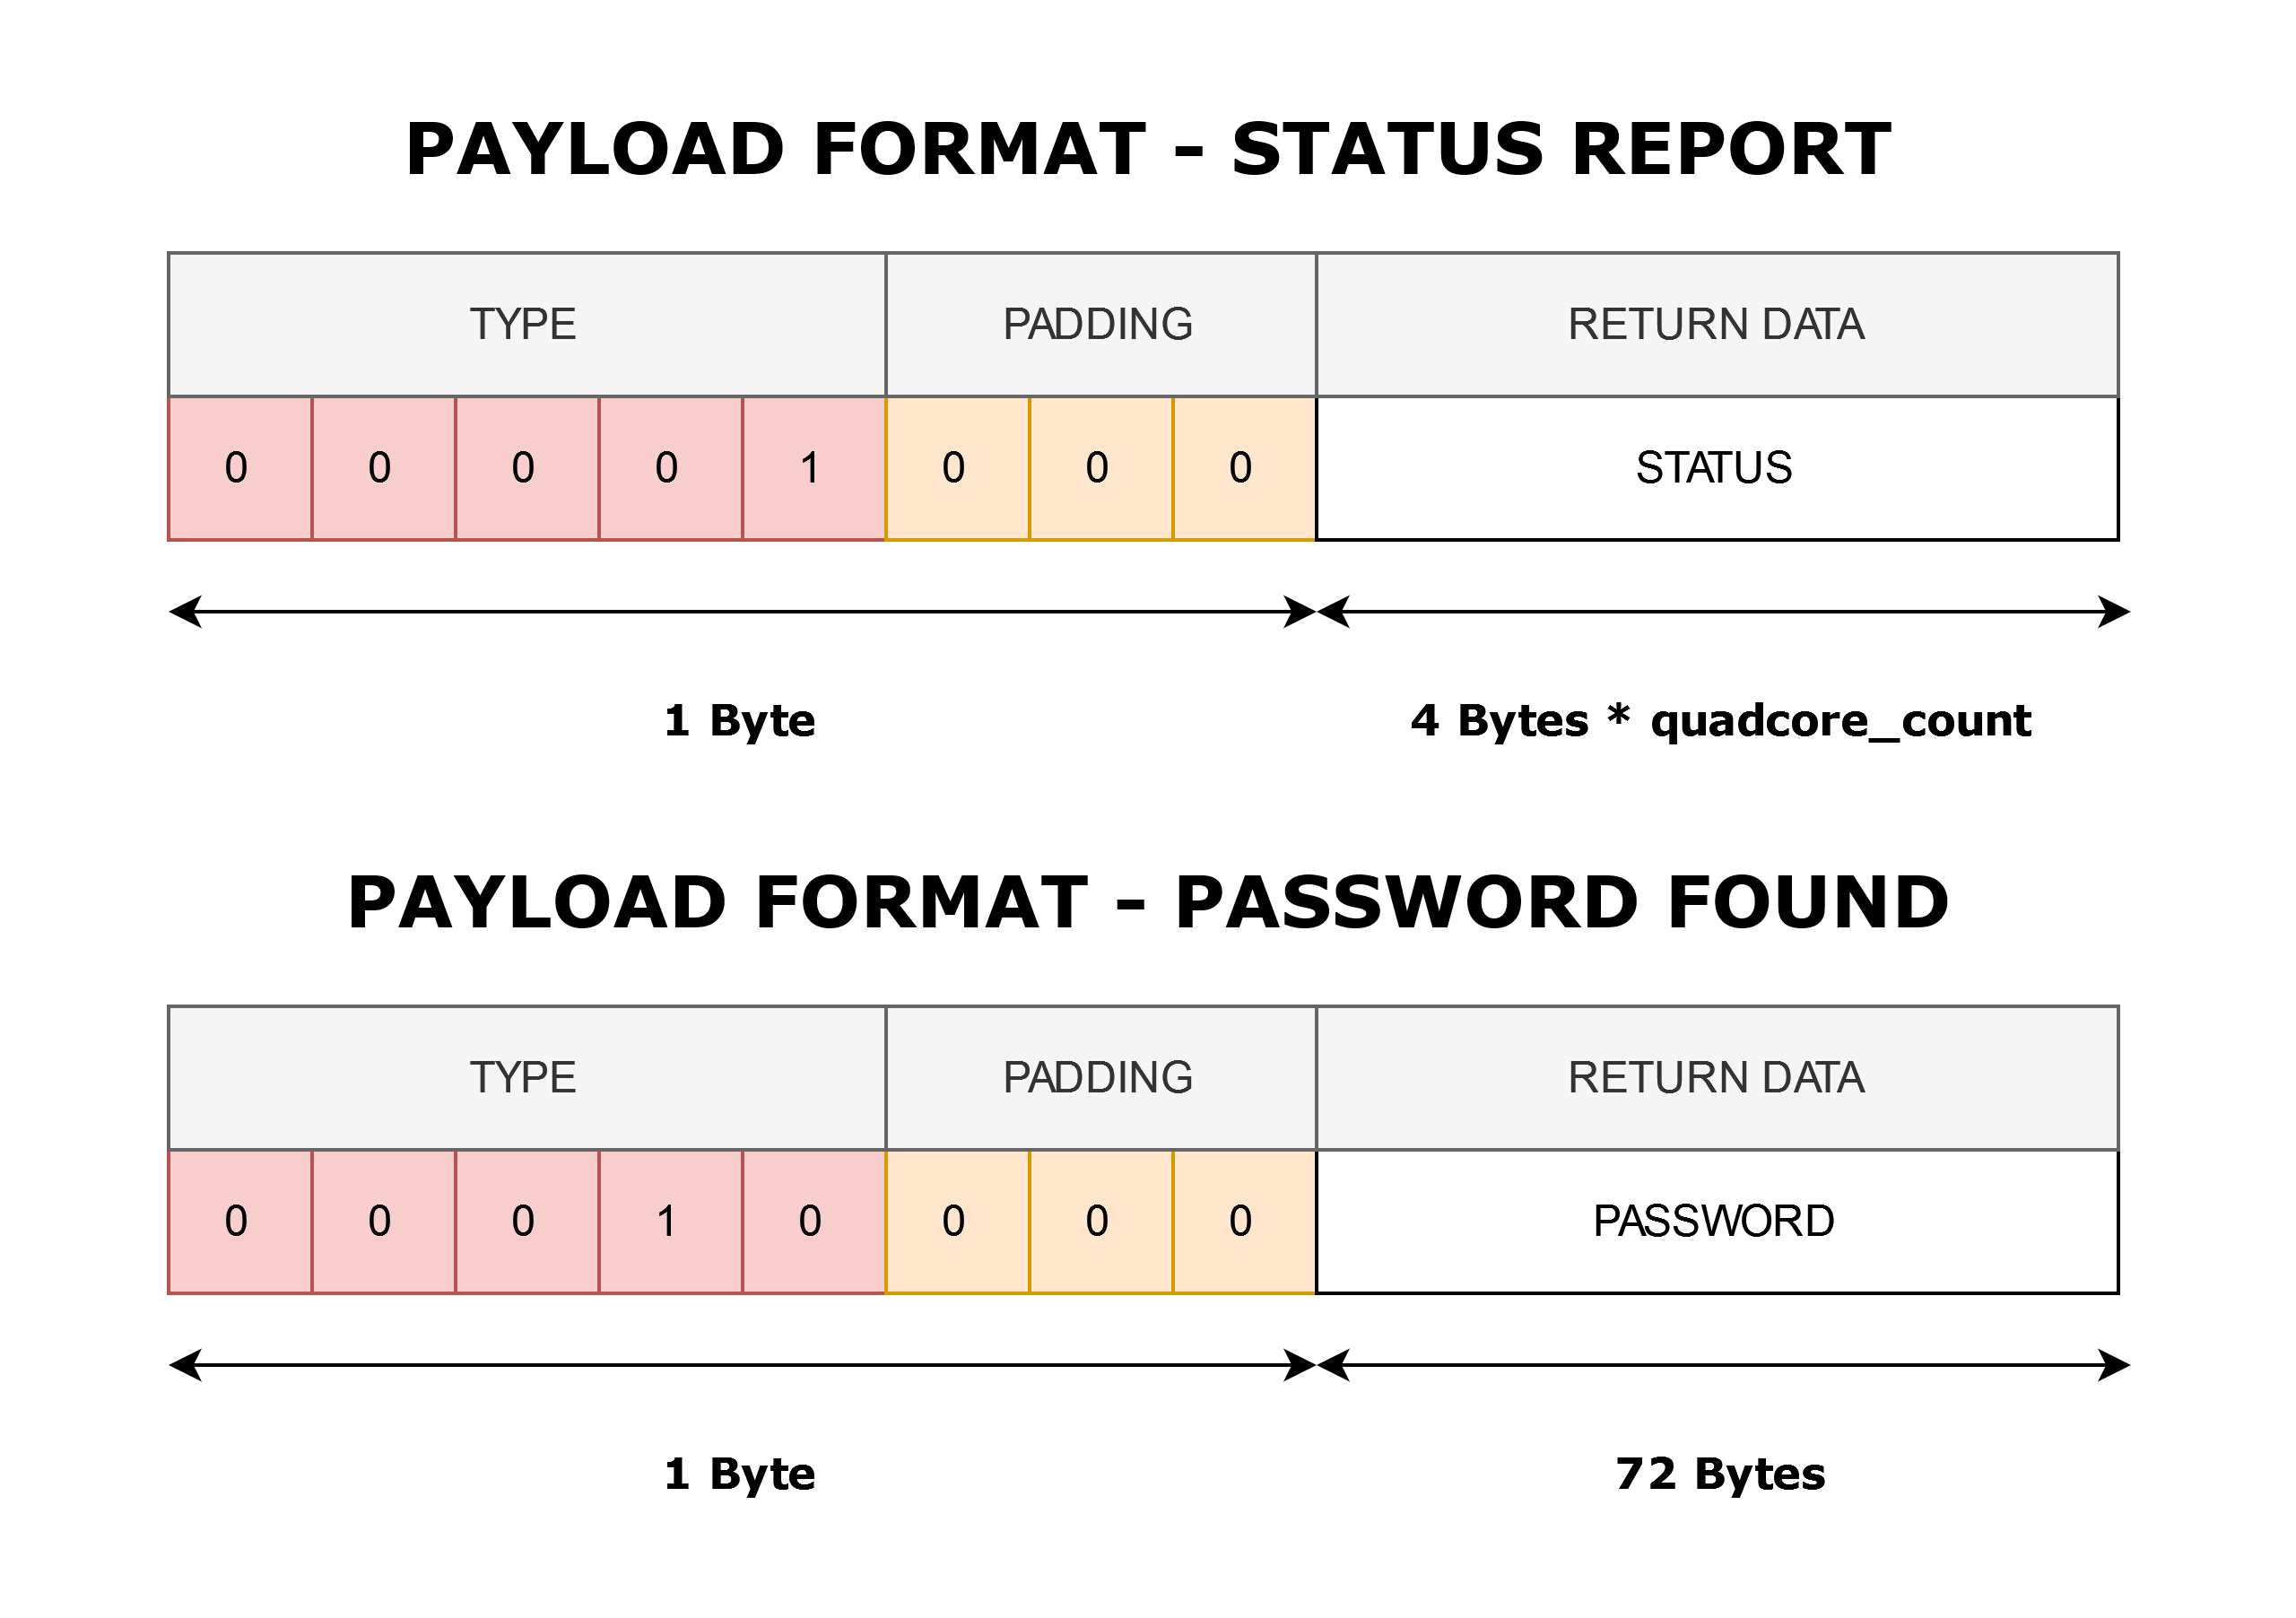
\includegraphics[width=0.7\linewidth]{uart_miso_payload_format}
	\caption[Format de paquet - MISO]{Format de paquet - MISO. Source : réalisé par Kandiah Abivarman}
	\label{fig:uart_miso_payload_format}
\end{figure}

\newpage

\section{Implémentation Solution UART}

\subsection{Architecture Logique}

Pour la partie implémentation, j’avais déjà un module \gls{uart} en \gls{vhdl} qui marchait et le bcrypt cracker fonctionnel lorsque réglage était codé en dur. 
Il fallait donc que je mette en place tout ce qui allait avoir entre l’interface \gls{uart} et le système d’attaque bcrypt, c’est-à-dire toute la partie gestion de paquet. 

Pour le module qui allait s’occuper des paquets, j’ai pensé à diviser cette partie en deux. 
Une première partie qui allait s’occuper de la réception des paquets, donc le décodage, la vérification et ressortir les données pour les quadcores. 
Puis une deuxième partie qui doit gérer toute la partie transmission des paquets de retours, de statut et du mot de passe trouvé. 
Les deux modules seront reliés de ce fait, lorsque il y aura un souci ou non avec un paquet reçu, le module de réception pourra avertir le module de transmission afin qu’il puisse envoyer le paquet de retours.

\begin{figure}[tbph!]
	\centering
	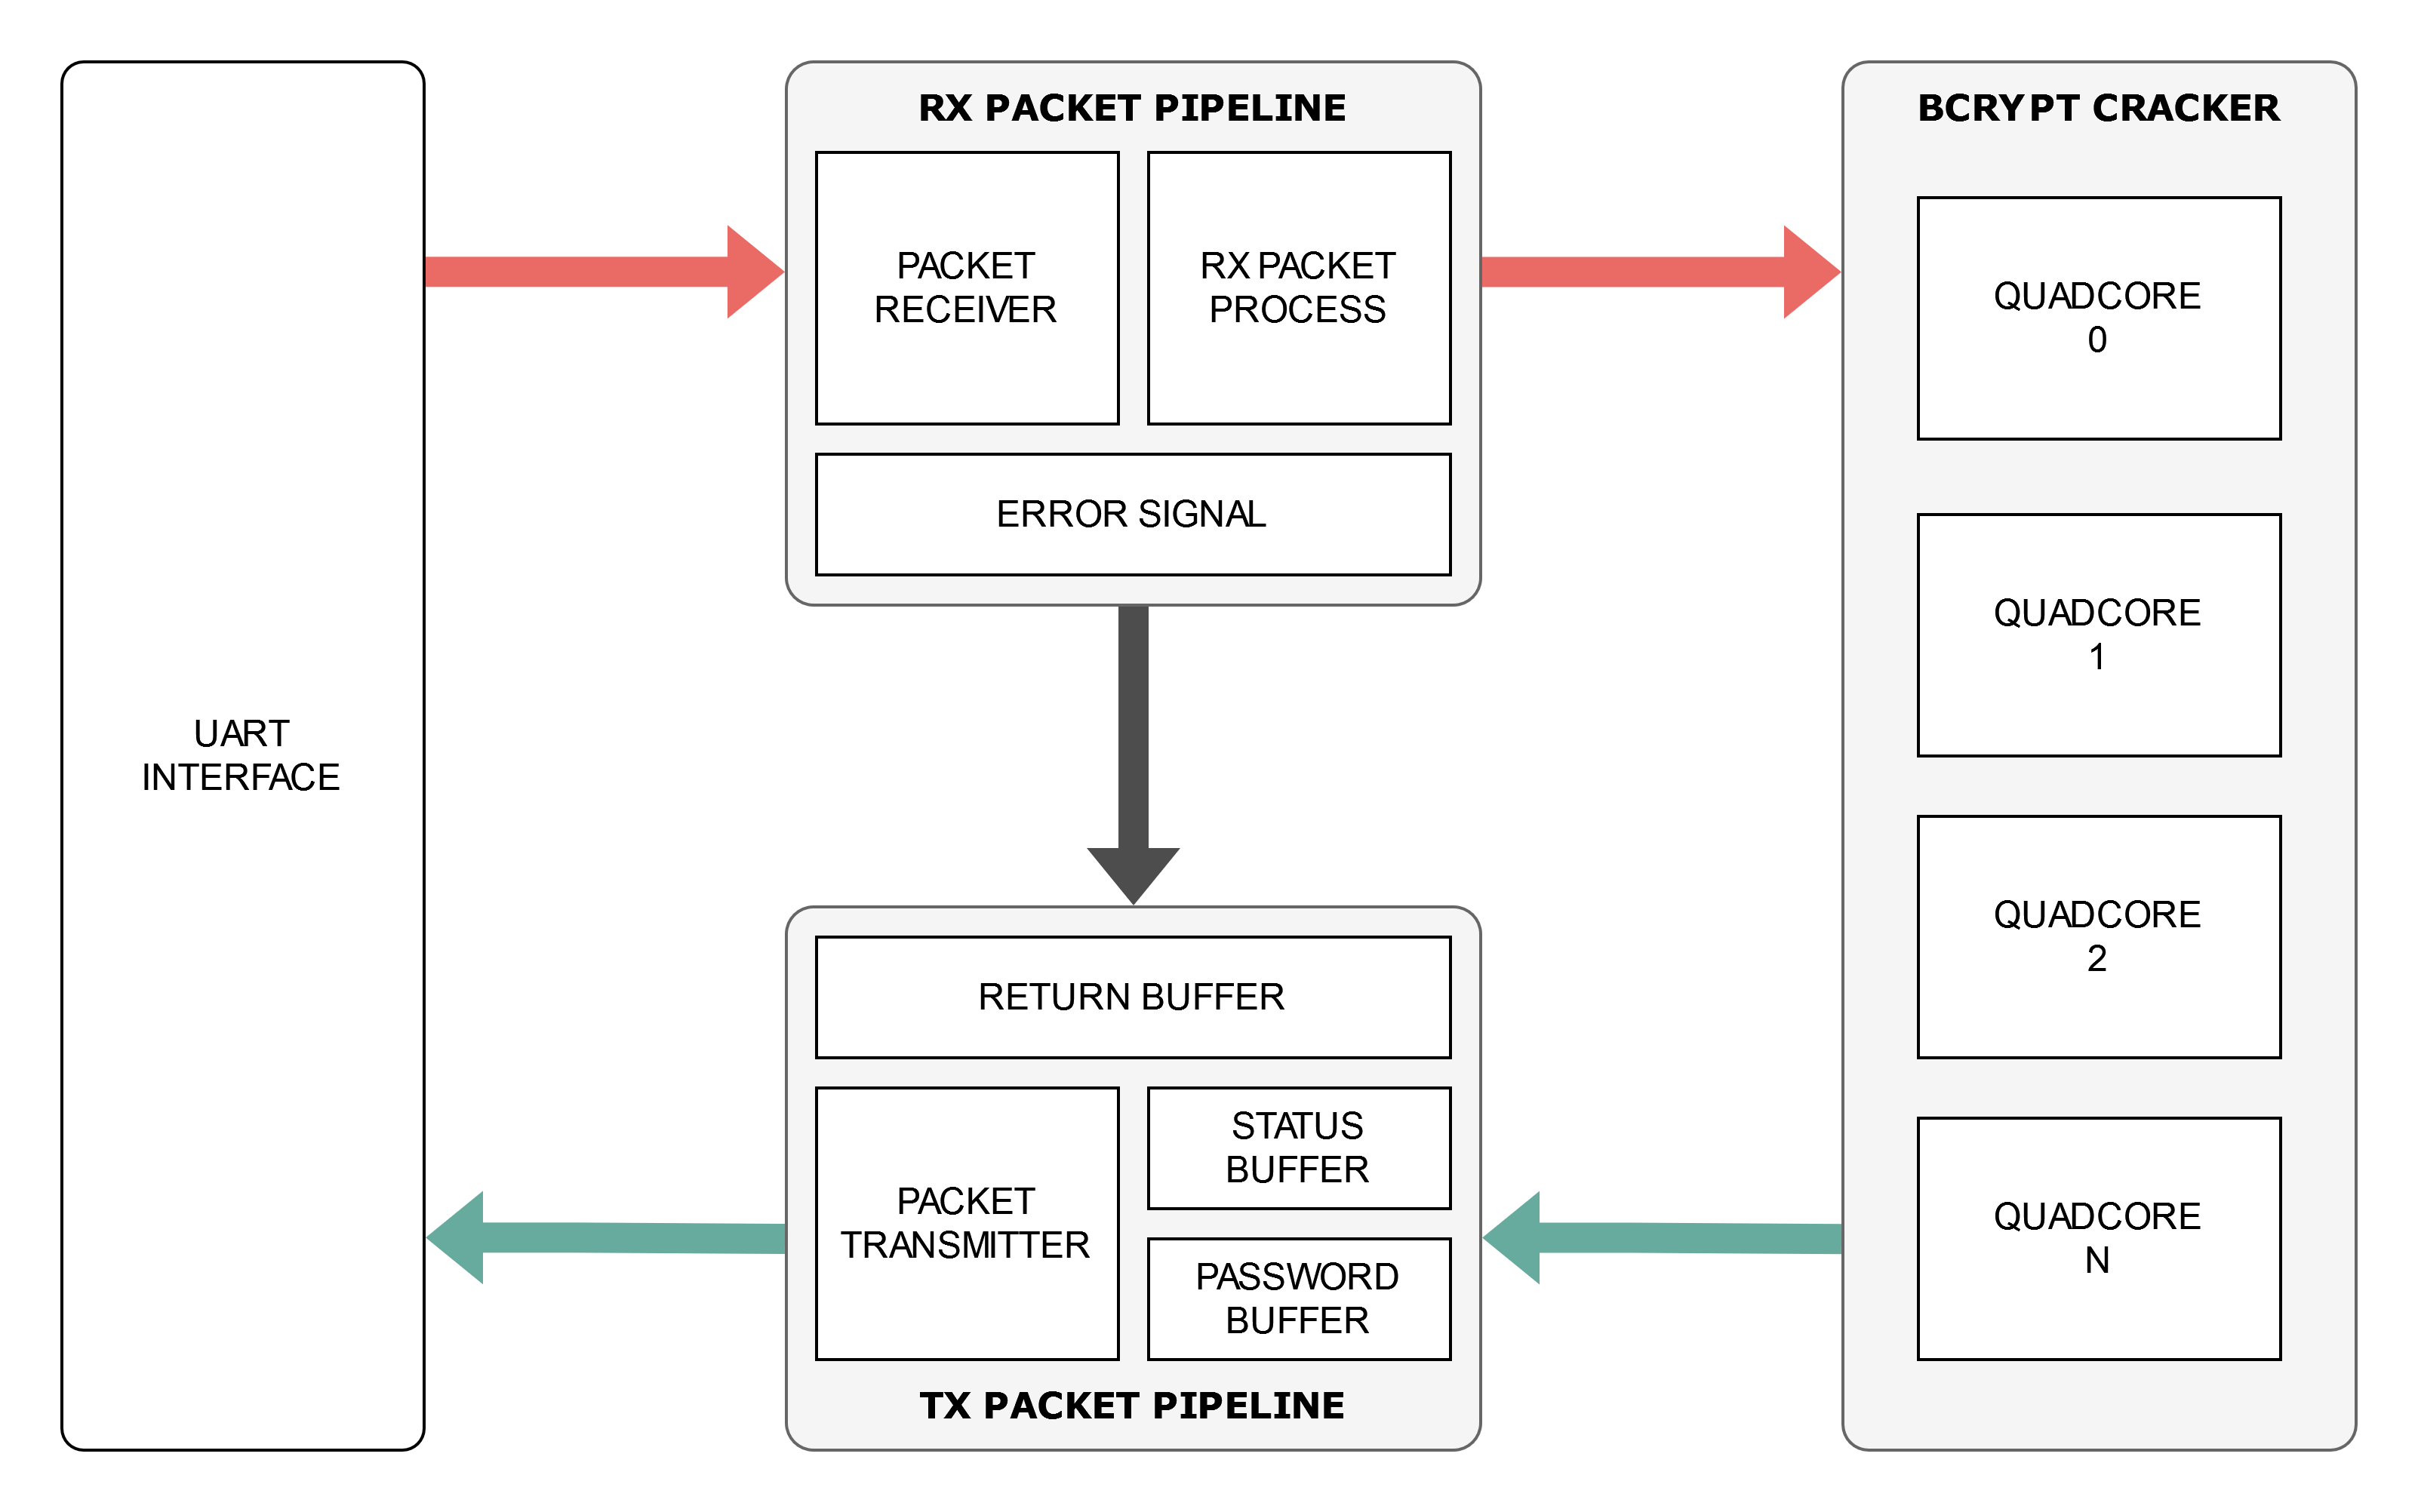
\includegraphics[width=0.7\linewidth]{uart_communication_protocol_top_rev2}
	\caption[Schéma système UART - FPGA]{Schéma système UART. Source : réalisé par Kandiah Abivarman}
	\label{fig:uart_top_schematics}
\end{figure}

J’ai aussi dû adapter le module bcrypt cracker et quadcore afin qu’il puisse marcher correctement avec l’architecture souhaitée.

\subsection{Modifications Bcrypt Cracker}

\subsection{Implémentation - MOSI}
\subsubsection{Module - Packet Receiver}
\subsubsection{Module - RX Packet Process}
\subsubsection{Module - RX Packet Pipeline}

\subsection{Implémentation - MISO}
\subsubsection{Module - Packet Transmitter}
\subsubsection{Module - TX Packet Pipeline}

\subsection{Tests}
\subsubsection{Simulations}
\subsubsection{Vérification Hardware}

\section{Interfacage Solution UART}

\newpage

\section{Description Solution PCIe}
\section{Implémentation Solution PCIe}
\section{Interfacage Solution PCIe}
